% !TEX TS-program = pdflatex
% !TEX encoding = UTF-8 Unicode

% This is a simple template for a LaTeX document using the "article" class.
% See "book", "report", "letter" for other types of document.

\documentclass[11pt]{article} % use larger type; default would be 10pt

\usepackage[utf8]{inputenc} % set input encoding (not needed with XeLaTeX)

%%% Examples of Article customizations
% These packages are optional, depending whether you want the features they provide.
% See the LaTeX Companion or other references for full information.

%%% PAGE DIMENSIONS
\usepackage{geometry} % to change the page dimensions
% \geometry{a4paper} % or letterpaper (US) or a5paper or....
% \geometry{margin=1in} % for example, change the margins to 2 inches all round
 \geometry{
 a4paper,
 total={180mm,267mm},
 left=15mm,
 top=15mm,
 }

% \geometry{landscape} % set up the page for landscape
%   read geometry.pdf for detailed page layout information

\usepackage{graphicx} % support the \includegraphics command and options

% \usepackage[parfill]{parskip} % Activate to begin paragraphs with an empty line rather than an indent

%%% PACKAGES
\usepackage{booktabs} % for much better looking tables
\usepackage{array} % for better arrays (eg matrices) in maths
\usepackage{paralist} % very flexible & customisable lists (eg. enumerate/itemize, etc.)
\usepackage{verbatim} % adds environment for commenting out blocks of text & for better verbatim
\usepackage{subfig} % make it possible to include more than one captioned figure/table in a single float
% These packages are all incorporated in the memoir class to one degree or another...

%%% HEADERS & FOOTERS
\usepackage{fancyhdr} % This should be set AFTER setting up the page geometry
\pagestyle{fancy} % options: empty , plain , fancy
\renewcommand{\headrulewidth}{0pt} % customise the layout...
\lhead{}\chead{}\rhead{}
\lfoot{}\cfoot{\thepage}\rfoot{}

%%% SECTION TITLE APPEARANCE
\usepackage{sectsty}
\allsectionsfont{\sffamily\mdseries\upshape} % (See the fntguide.pdf for font help)
% (This matches ConTeXt defaults)

%%% ToC (table of contents) APPEARANCE
\usepackage[nottoc,notlof,notlot]{tocbibind} % Put the bibliography in the ToC
\usepackage[titles,subfigure]{tocloft} % Alter the style of the Table of Contents
\renewcommand{\cftsecfont}{\rmfamily\mdseries\upshape}
\renewcommand{\cftsecpagefont}{\rmfamily\mdseries\upshape} % No bold!

%%% END Article customizations
\usepackage{amsmath}
\usepackage{hyperref}
\usepackage{float}  
\usepackage{multirow}


%%% The "real" document content comes below...



\title{Starbucks capstone project}
\author{Thomas Heinemann}
%\date{} % Activate to display a given date or no date (if empty),
         % otherwise the current date is printed 

\begin{document}
\maketitle

\section{Project overview}

This is a recommendation engine project proposed by Starbucks to find out which demographic groups of customers respond best to certain types of offers. The underlying data sets include transactional and customer data, as well as information about the types of offers sent. The full set
of files, including the main Jupyter file with the detailed task, can be found at \cite{a}.
In addition, an approach for a simpler version of such a problem can be found here \cite{b}.
%\cite[1]{rfewf}


\begin{thebibliography}{2}

\bibitem{a} All project files: {\scriptsize \url{https://github.com/thomasheinemann/starbucks_promotion_type_exercise/}}

\bibitem{b} Simpler version of this project: {\scriptsize\url{https://github.com/thomasheinemann/starbucks_promotion_exercise/}}



\end{thebibliography}

\section{Introduction}
To begin with we first present the original introduction and task (the full description is here \cite{a}):


\begin{quote}
\begin{em}
This data set contains simulated data that mimics customer behavior on the Starbucks rewards mobile app. Once every few days, Starbucks sends out an offer to users of the mobile app. An offer can be merely an advertisement for a drink or an actual offer such as a discount or BOGO (buy one get one free). Some users might not receive any offer during certain weeks. 

Not all users receive the same offer, and that is the challenge to solve with this data set.

Your task is to combine transaction, demographic and offer data to determine which demographic groups respond best to which offer type. This data set is a simplified version of the real Starbucks app because the underlying simulator only has one product whereas Starbucks actually sells dozens of products.

Every offer has a validity period before the offer expires. As an example, a BOGO offer might be valid for only 5 days. You'll see in the data set that informational offers have a validity period even though these ads are merely providing information about a product; for example, if an informational offer has 7 days of validity, you can assume the customer is feeling the influence of the offer for 7 days after receiving the advertisement.

You'll be given transactional data showing user purchases made on the app including the timestamp of purchase and the amount of money spent on a purchase. This transactional data also has a record for each offer that a user receives as well as a record for when a user actually views the offer. There are also records for when a user completes an offer. 

Keep in mind as well that someone using the app might make a purchase through the app without having received an offer or seen an offer.
\end{em}
\end{quote}

So how do we proceed?
A simple statistical evaluation based on the frequency of offer completions or views per customer may not work as we do not have huge data sets for each person with and without receiving, viewing and completing a considered offer type. Also, a customer being researched may not have exactly the same profile as those being provided.
We therefore improve the statistics by reducing the value set of the customer profile data.
However, this is not enough, so we train models to predict as accurately as possible whether the customer is worth promoting or not.
The advantage of this is that these models also make good use of information from other more or less similar customer profiles.

In the following sections, we provide definitions, present the modelling approach, summarise the results for each type of offer and conclude with our main findings in the conclusion section.


\section{Definitions}
\textbf{Main offer types to be considered:}
\begin{itemize}
\item BOGO (buy one get one free) offer: If the customer buys the praised product of this offer then this person gets the same product on top for free.
\item discount offer: If the customer spends a certain amount then this person receives a discount.
\item informational offer: These offers just show the customer an advertisement for a product, e.g., a drink. In the given data, however, there is no offer completion record.
For this purpose, we define an offer instance as "completed" if the hourly spend exceeds that of an no-offer instance, and vice versa.
\end{itemize}
\noindent\textbf{Offer instance:} 
An offer sent for one specific customer, at one specific time (offer\_received\_time). So each offer instance is addressed with the key \textbf{[offer\_id, person, offer\_received\_time]} which is found being unique.
No-offer times of a customer are treated as "no-offer" offer instances and addressed with [offer\_id="no offer", person, offer\_received\_time=0].
\\
\\
\noindent\textbf{Offer events:} 
\begin{itemize}
\item offer received
\item offer viewed (can also happen after offer is completed or no longer valid)
\item transaction = the customer makes a transaction of a certain amount (can happen during an offer or a "no-offer" time)
\item offer completed = the difficulty challenged by the offer has been overcome with the current transaction
\end{itemize}
\noindent\textbf{Offer event times:} 
Times of the  events above are further denoted as "offer\_received\_time", "offer\_viewed\_time", "transaction\_time", and "offer\_completed\_time".
\\
\\
\textbf{Offer event record (OER): }An OER consists of an offer received event, a possible offer viewed or completed event, and all transaction events associated with a specific offer instance.
Similar to each offer instance, each OER is addressed using the unique key [offer\_id, person, offer\_received\_time].
For each person we also define one OER associated with no offer times which is addressed with [offer\_id="no offer", person, offer\_received\_time=0].
Each OER has an offer validation interval starting at its offer\_received\_time and ending at $$\mathrm{offer\_time\_out}=\mathrm{offer\_received\_time}+24 \times \mathrm{duration}.$$ 
The duration is the maximum offer-specific time interval in days during which the offer can be valid if not completed earlier.
\\
\\
\textbf{States of an offer instance}: 
\\
Each offer instance is characterised by the binary state variables "promoted", "viewed" and "completed".
Their calculation requires the corresponding OER and is shown in the following table.
\\
\\
\begin{tabular}{|c||c|c|c|c|}
 \hline
\textbf{state variables of an offer instance} & \textbf{calculation in terms of logical expressions} \\ 
\hline
\hline
promoted & offer\_id $\ne$ "no offer"\\ 
\hline
\multirow{ 2}{*}{viewed} &  $\mathrm{offer\_viewed\_time} \le \mathrm{offer\_end\_time}$\\ 
&  with: $ \mathrm{offer\_end\_time}=Min(\mathrm{offer\_time\_out},\mathrm{ offer\_completed\_time})$\\ 
\hline
completed & $\mathrm{ offer\_completed\_time} \le \mathrm{offer\_time\_out} $ \\ 
\hline
\end{tabular}
\\
\\
\\
\textbf{Consumption during offer:}
It is a quantity related to an OER.
It is defined as the sum of all transactions made in an OER where each transaction lies in the time interval [offer\_received\_time, offer\_time\_out].


\section{Modeling approach}
\subsection{Data flow}
The data flow along our prediction pipeline starts with the original customer profile attributes and ends with a decision on whether or not to promote that person. The first step is to get rid of NaN values and introduce categorical variables for the gender attribute. In the second step, model 1 predicts an early viewing probability, which is used to sort out "lazy viewers".  To predict the final decision to send the offer, in step 3 we used model 2, which is fitted separately for each type of offer.
\begin{figure}[H]
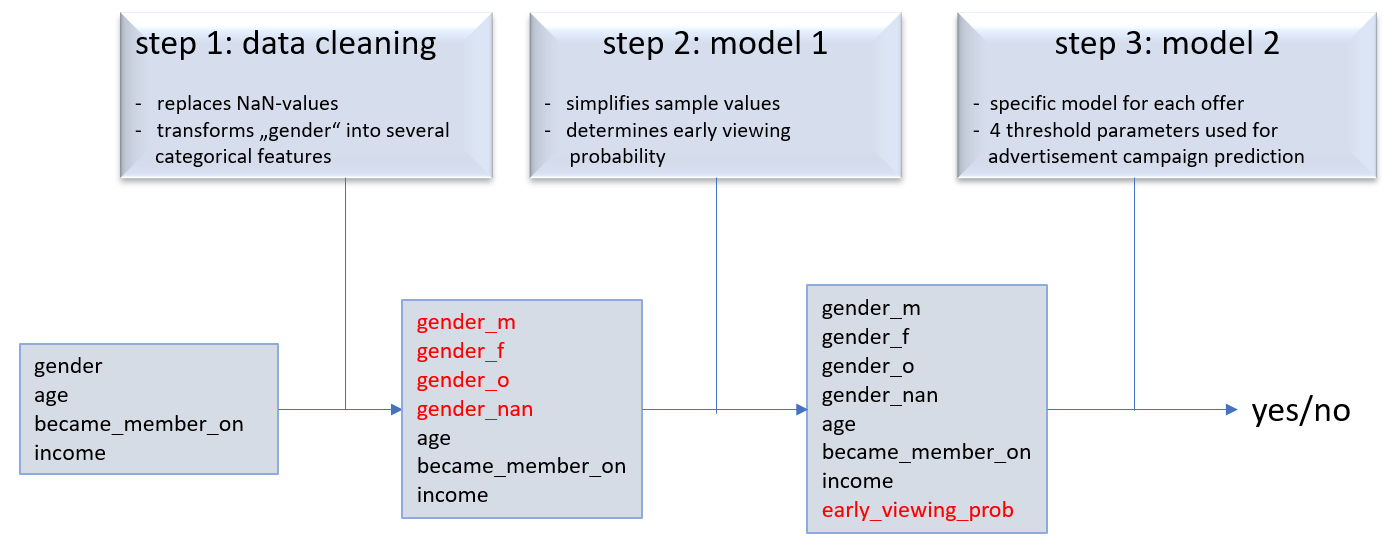
\includegraphics[width=0.95\textwidth]{dataflow.png}
\caption{Data flow showing a prediction  pipeline for the customer profile attributes  "gender", "age", "became\_member\_on", "income" to a "yes/no" prediction for an advertisement campaign. For each offer type a differently fitted version of model 2 is used. Models 1 and 2 were fitted using customer profile attributes and customers' offer event records (OERs).}
\end{figure}

\subsection{Step 1: data preparation}
The customer profile data is first subjected to a NaN-value treatmet for the income.
In particular, customers who do not report an income, are marked as having an income of -10,000 dollars.
Another issue treated in this step is the gender attribute which is categorical without order and therefore split into one-hot encoded attributes for each class label, resulting in "gender\_m", "gender\_f", "gender\_o",  and "gender\_nan" (indicating if no gender is provided).




\subsection{Step 2: model 1}
Model 1 has the task of simplifying the value sets of the customers' integer features "age", "become\_member\_on" and "income" using a transformer to achieve 10 year steps for the "age", 1 year steps for "become\_member\_on" and 10,000 dollar steps for "income".
Then, in a second transformation, a test-set customer receives, within the framework of model 1, an early viewing probability encoded in the attribute, "early\_viewing\_prob" (probability that the offer will be viewed within 48 h).
This transformer also produces viewing preference information with the self-explanatory attributes "early\_viewing\_pref" and "late\_viewing\_pref"' to predict whether the customer prefers to view within 48 hours, prefers to view after 48 hours or does not tend to view at all.
These attributes are not used as feature variables in subsequent steps of the pipeline, as they are only predicted from the demographic attributes, but are useful for supporting the visualisation of a customer's demographics in the results section.
The underlying model of the second transformer is fitted with all the cleaned customer profile data from the profile training set, together with information about their OERs. The offer instances to be considered include only the customers' non-overlapping offer instances. This restriction was chosen because multi-offer effects can be quite complex and would be a further step of investigation that would likely require more data.


\subsection{Step 3: model 2 (offer specific model)}

In this step, an offer-specific model comes into play. Accordingly, a separate instance of this model is used for each offer type.
The model itself uses cleansed customer profile data and all the customers' OERs of non-overlapping offer instances of the considered offer type and their corresponding no-offer OERs.
The "offer completion" states for the no-offer instances are calculated in this model as if the customer had been promoted with the offer type considered in this model.
To be precise, a difficulty had to be overcome that scales with the ratio between the no-offer and the offer duration.

Regarding the states of the offer instances, we generally distinguish six since an offer can be  sent or not, can be viewed (if a promotion exists) or not, and completed or not.
A grouping of these six classifications into four different labels forms the basis of the current model and is shown in the table below.

\begin{center}
{\Large
\begin{tabular}{|c||c|c|c|c|}
 \hline
&\multicolumn{3}{c|}{  \textbf{states of offer instances}}\\
 \textbf{label} & promoted & viewed & completed \\ 
\hline
\hline
I & yes & yes & yes \\ 
\hline
\multirow{ 2}{*}{II} & no & no & yes \\ 
 & yes & no & yes \\ 
\hline
III & yes & yes & no \\ 
\hline
\multirow{ 2}{*}{IV} &no & no & no \\ 
 & yes & no & no \\ 
 \hline
\end{tabular}
}
\end{center}

The aim of Model 2 is to make use of the upper 4-label classification of offer instance states to predict customers who only complete the offer when viewed.
Ideally, these customers will only have offers with states labelled I and IV, respectively. Fig. \ref{fig:venn2} shows a Venn diagram depicting ideal customer sets along with the one we are interested in. We hereby define an ideal customer as one for whom the offer completion status is solely dependent on the viewing status, or is even independent of the latter.
This definition leads to the four different types of ideal customers shown in the figure below.
\begin{figure}[H]
\begin{center}
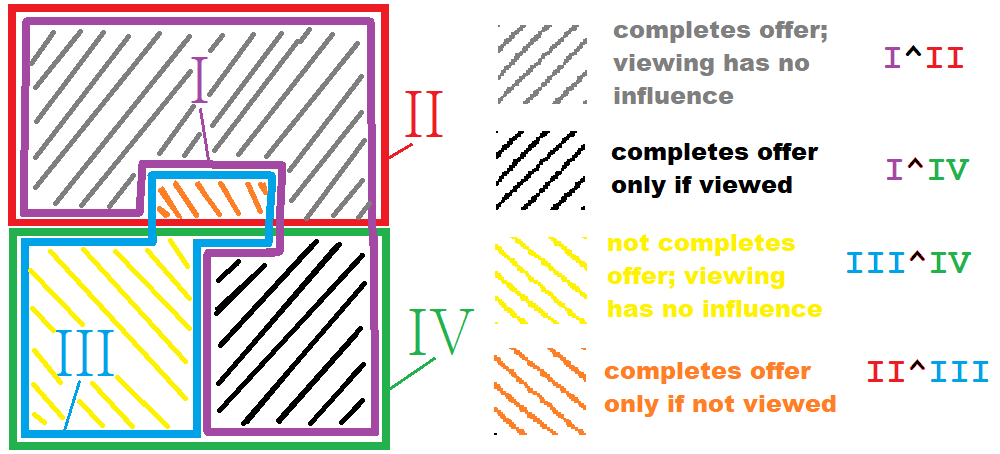
\includegraphics[width=0.7\textwidth]{venn_diagram2.png}
\caption{\label{fig:venn2}A Venn diagram is shown, representing a grouping of ideal customers into four disjunct sets filled with differently colored diagonal stripes. In each set there are only two different offer instance state labels (represented by Roman numbers). 
}
\end{center}
\end{figure}

Unfortunately, our customers are not ideal, so each customer will behave differently in relation to each individual offer instance.
Therefore, the only way we can predict what behaviour the customer is most likely to reveal is by assuming a correlation between the customer's profile and the states of their offer instances.

In order to determine whether a customer will "complete the offer only if viewed", we create one predictor to distinguish between customer profiles with states labelled II vs. those with states labelled IV, and analogously a second to distinguish between I vs. III.
Using their prediction probabilities for both label I and label IV customers, we can get a good estimate of the black-striped area. To do this, the threshold parameters $p_1$ and $p_2$ must be exceeded by both prediction probabilities.


However, some customers are actually discouraged from buying when they see an ad (see orange-striped area). These customers are not in the black-striped area, but since the boundaries are fuzzy, we
also included a third predictor (with threshold parameter $p_3$) that distinguishes between customer sets with labels I $\cup$ IV vs. II $\cup$ III. This allows separate tuning of the boundary between the orange and black striped area and the boundary between the orange and grey striped area. In addition, we have implemented a fourth threshold parameter $p_4$ for the early viewing probability determined in model 1 to weed out lazy viewers in the result set.
This can prevent too many customers from being unknowingly rewarded.

The threshold parameters are optimised on a hyperparameter grid for each model 2 instance using a 3-fold cross-validation procedure.
The scoring metrics for the validation sets and the test set used for every model 2 instance are defined below.

\subsection{Scoring metric}
The scoring metric was chosen to take into account two important aspects.
Firstly, we want to maximise the number of customers who complete an offer when they receive it. The underlying metric to be maximised is the "incremental response rate" ("irr").
On the other hand, we aim to gain consumption by maximising a shifted version of "net incremental revenue" ("nir").
This prevents our recommendation algorithm from promoting too many customers whose rewards make them spend less because they are too satisfied.
As a scoring metric, we therefore used a compromise that is a product of the two previous metrics, i.e.
\begin{align}
\text{scoring metric}= irr \times nir
\end{align}
Both metrics are defined in the following.
%
\\
\\
\text{\bf Incremental response rate "irr" (for offer type X):}
\begin{align}
irr=\frac{ n_{prom,compl} }{ n_{prom}} &-\frac{ n_{no\ prom,compl} }{ n_{no\ prom}}
\\
\nonumber\\
n_{prom,compl}:& \text{\ number of instances of offer type X which are completed}\nonumber
\\
n_{prom}:& \text{\ number of instances of offer type X}\nonumber
\\
n_{no\ prom,compl}:& \text{\ number of no-offer instances whose consumption rate would have completed}\nonumber
\\
& \text{an offer of offer type X}\nonumber
\\
n_{no\ prom}:& \text{\ number of no-offer instances}\nonumber
\end{align}
\text{\bf Shifted net incremental  revenew  "nir" (for offer type X):}
We take the sum of the consumption of completed offers (of offer type X) minus the sum of the consumption of no-offer instances whose consumption rate would satisfy an offer completion event of offer type X.
Each consumption is normalised by its corresponding offer/no-offer duration. The function of the shift is to take care of the imbalanced data sets of completed offer instances vs. completed no-offer ones.
\begin{align}
nir=& \sum_{\substack{i \in \text{ "completed" offer}\\ \text{instances in}\\ \text{ test set}}} \frac{ \text{consumption(i) }}{ \text{duration(i) }} -   \sum_{\substack{k \in \text{ "completed" } \\ \text{no-offer instances  }\\ \text{in test set}}} \frac{  \text{consumption(k) }}{ \text{ duration(k) }}-\text{shift}\cdot  n_{\text{test}}
\\
\nonumber\\
 \text{consumption }(x):& \text{\ consumption during offer/no-offer instance x}\nonumber\\ 
 \text{duration }(x):& \text{\ duration of offer/no-offer instance x}\nonumber\\ 
 n_{\text{test}}:& \text{\ number of all offer/no-offer instances (in the test set)}\nonumber\\ 
 n_{\text{train}}:& \text{\ number of all offer/no-offer instances (in the training set)}\nonumber\\ 
 \text{shift}=& {\tiny   \frac{1}{ n_{\text{training}}}   \left(
 \sum_{\substack{i \in \text{ "completed" offer}\\ \text{instances in}\\ \text{ training set}}} \frac{ \text{consumption(i) }}{ \text{duration(i) }} -   \sum_{\substack{k \in \text{ "completed" } \\ \text{no-offer instances  }\\ \text{in training set}}} \frac{  \text{consumption(k) }}{ \text{ duration(k) }}  \right)    }\nonumber
\end{align}




\section{Results}



\subsection{Cluster analysis for all customers in the test set}
In this section we present a cluster analysis of all customers using five histograms covering gender, income, age, membership begin year and viewing preference, with the bin counts for each cluster stacked on top of each other using different colours. Clustering was performed in a five-dimensional space spanned by all of the above demographic attributes, each represented by a histogram.
The optimal number of clusters was determined using the kmeans++ algorithm with the help of the silhoutte score and is limited here to five for simplicity.


\begin{figure}[H]
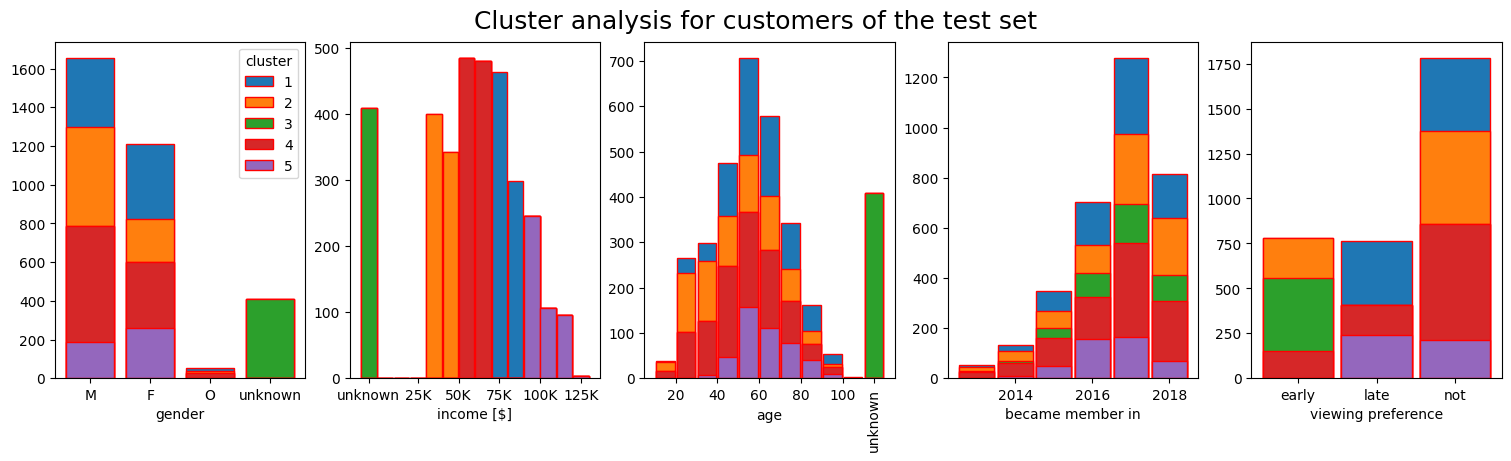
\includegraphics[width=1\textwidth]{results/results_test_set.png}
\caption{Cluster analysis for all customers in the test set using 5 clusters. In terms of clustering, we can see that people who do not provide information on gender, income and age are all early viewers. 
Customers earning more than \$70,000 are slightly dominated by women. Those earning more than \$90,000 are not under 40 years old and do not tend to view offers within two days.}
\end{figure}

\subsection{Analyzing the promotion strategy for each offer type}
In this subsection we briefly analyse, for each offer type (grouped by main offer types), which customers we would and would not recommend for a promotion using the strategy presented here.
Each figure represents the results of one offer type analysis and consists of three rows of graphs covering the demographic information of gender, income, age, membership begin year and viewing preference.
The top row of graphs shows data for all customers and highlights the customers who should be promoted according to the strategy found.
The middle row contains data only for customers to be promoted, while the bottom row contains data only for customers not to be promoted.
The customer demographics in the corresponding histograms have been clustered in the five-dimensional space spanned by all the aforementioned demographic attributes. Clustering was performed separately for target and non-target customers. In each analysis, the values for the "irr" and "nir" metrics, the threshold parameters of model 2 ($p_1, p_2, p_3, p_4$), as well as the metric score and the target (non-target) to test set ratio or 'coverage' of all test set customers are shown.
The values for the threshold parameters shown in this investigation, each multiplied by 100, refer to the percentile of the corresponding prediction probability values determined in the training set.
The following hyperparameter grid was used for optimizing $p_1,\dots, p_4$: $p_1,\dots, p_3 \in (0, 0.25, 0.5, 0.75, 1)$ and for $p_4 \in (0,0.1,\dots,0.9)$.
\subsubsection{Diagrams for BOGO offers}

\begin{figure}[H]
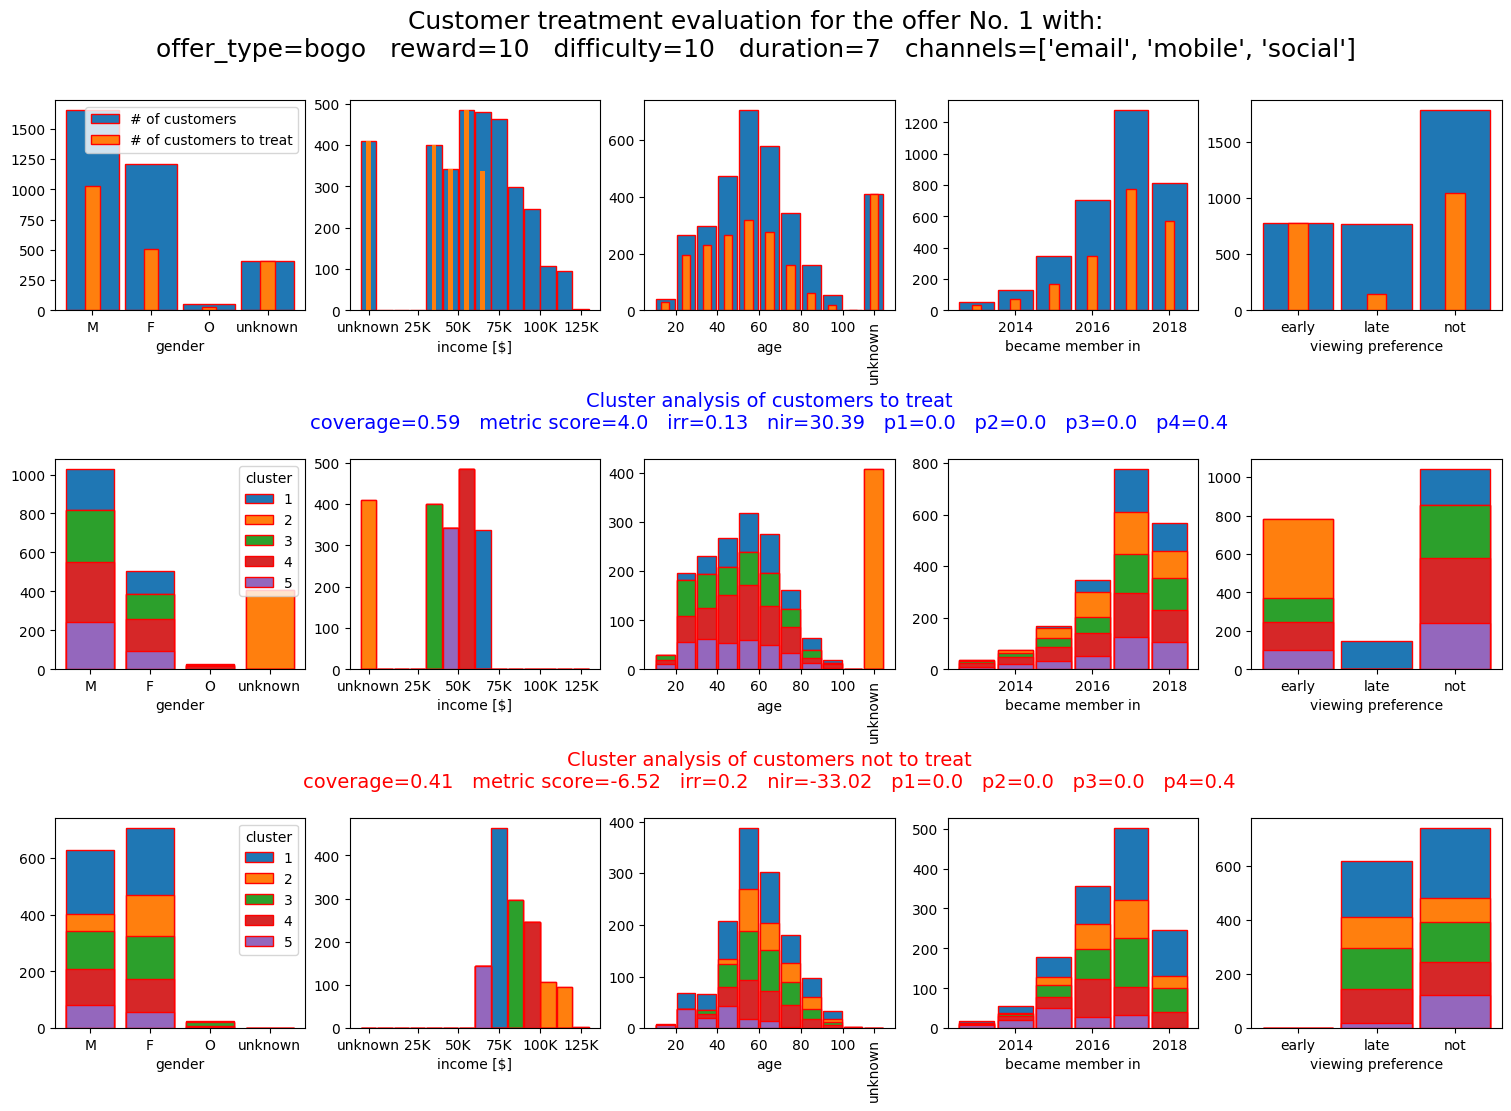
\includegraphics[height=0.5\textheight]{results/results1.png}
\caption{Customers with  incomes up to \$70,000 are worth targeting with this offer.  Those who do not provide demographic information should be included as well. The considered customers tend to view early or rather not. }
\end{figure}
\begin{figure}[H]
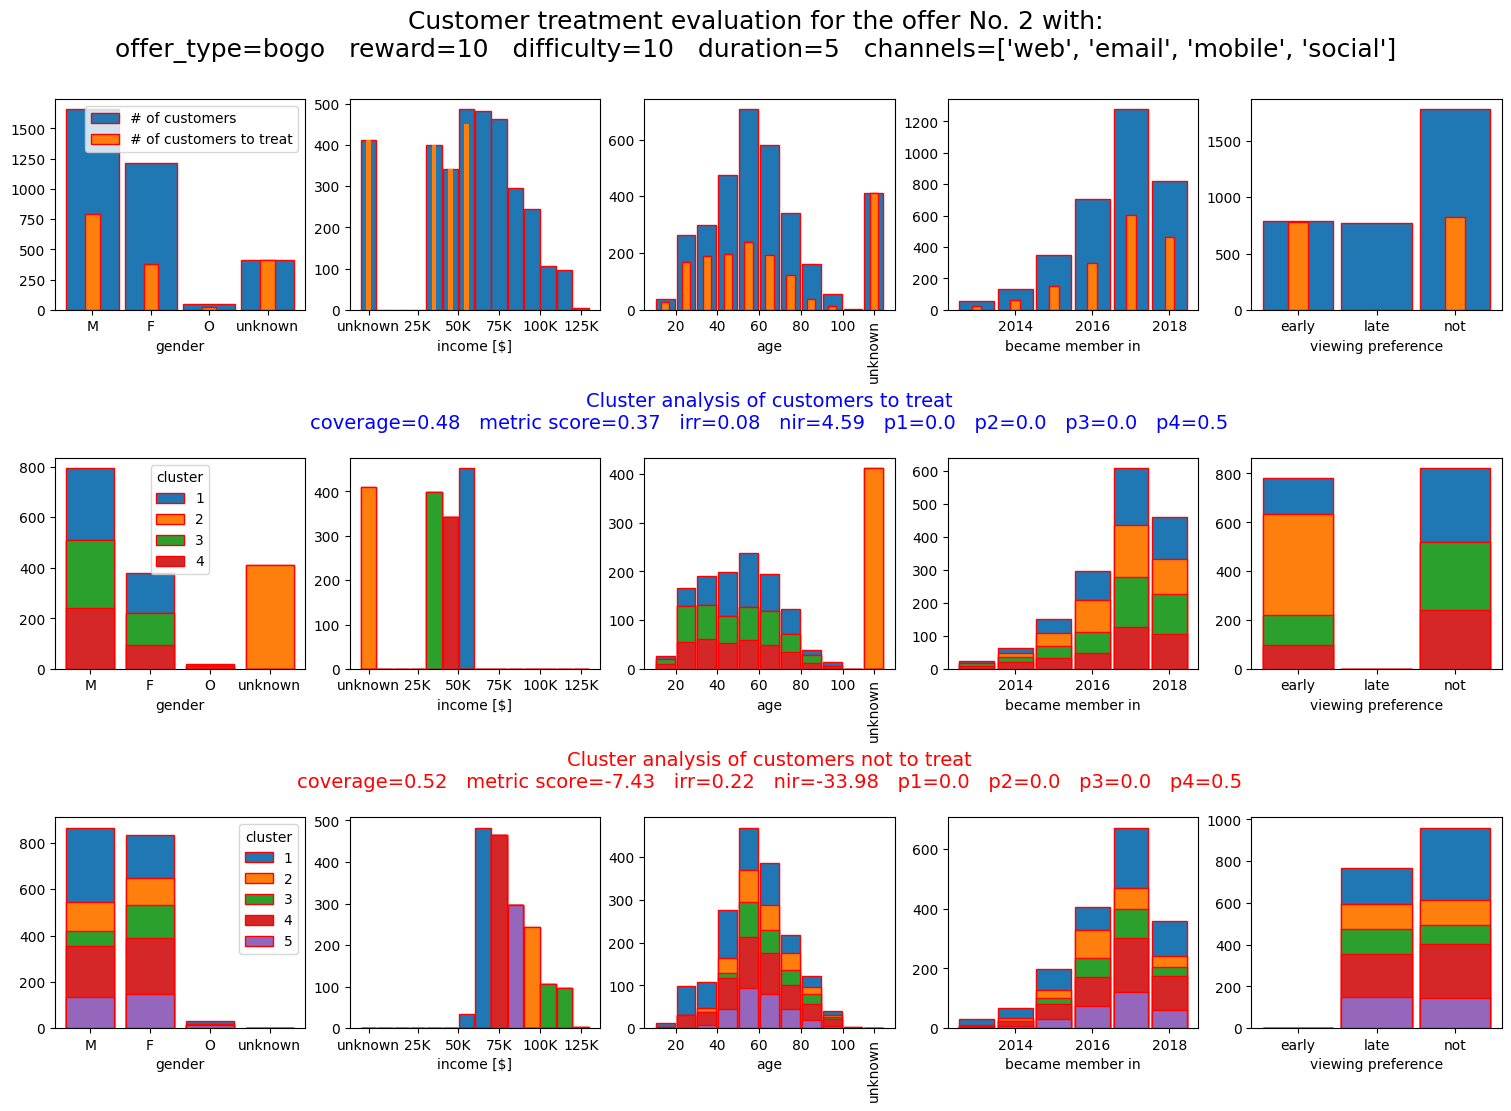
\includegraphics[height=0.5\textheight]{results/results2.png}
\caption{Customers with  incomes up to \$60,000 are worth targeting with this offer.  Those who do not provide demographic information should be included as well. The considered customers tend to view early or rather not. }
\end{figure}
\begin{figure}[H]
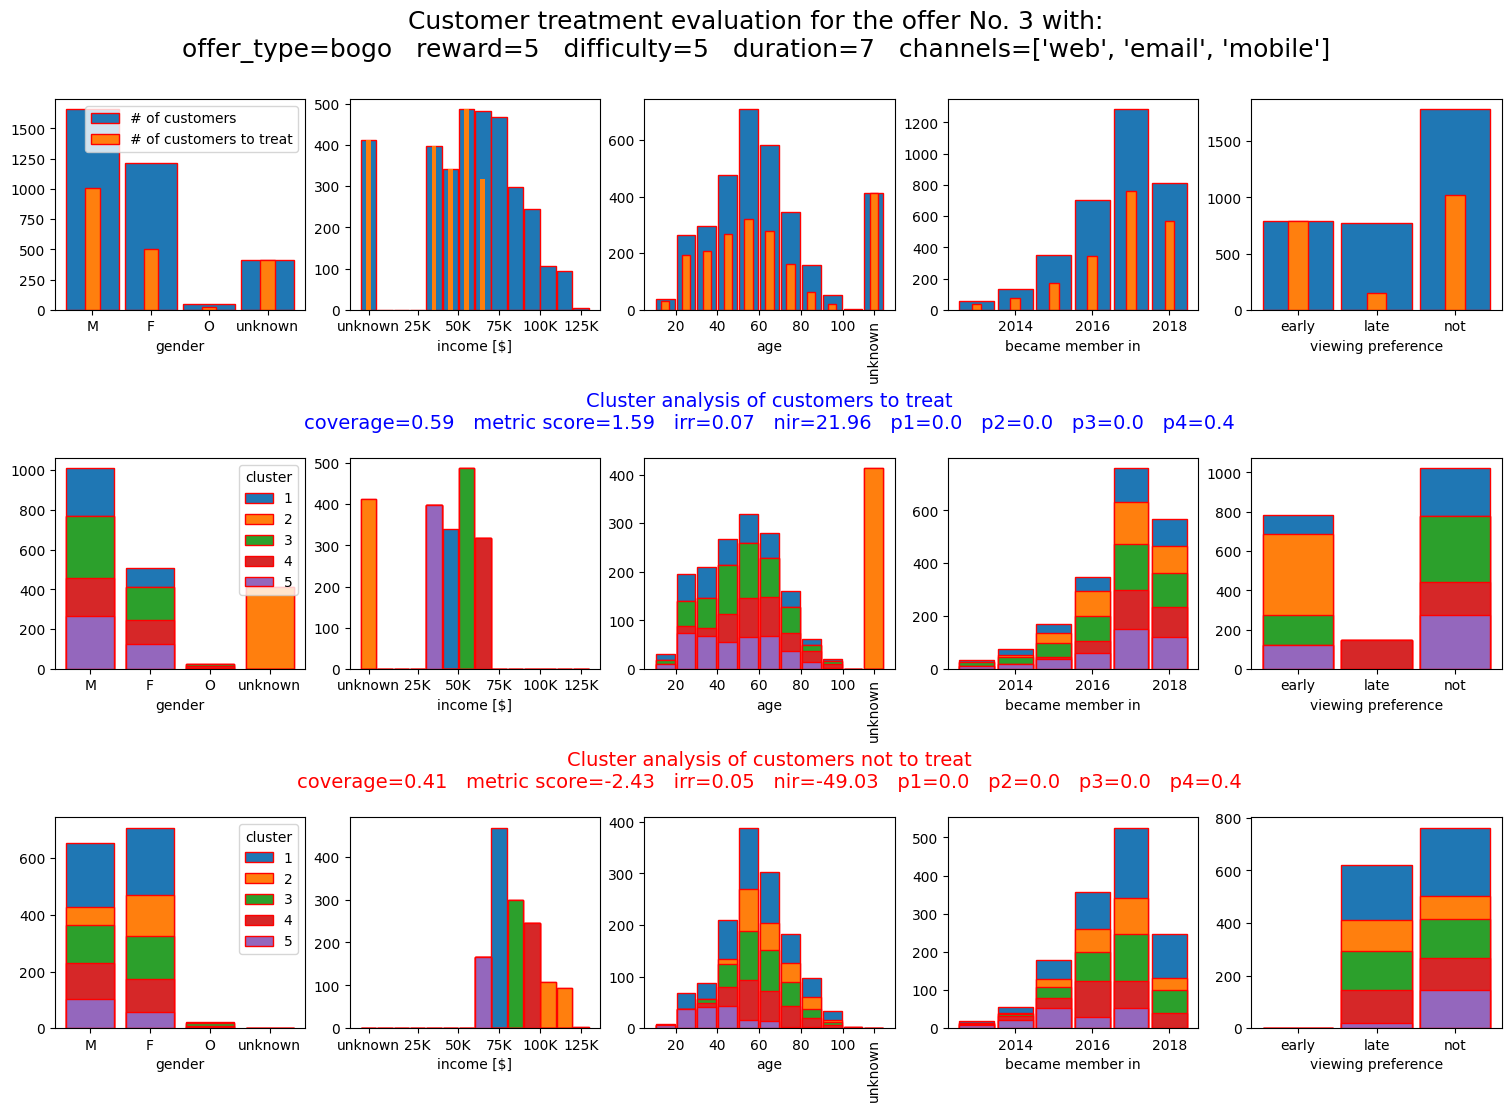
\includegraphics[height=0.5\textheight]{results/results3.png}
\caption{Customers worth targeting with this offer are basically the same as in offer type 1. However, this offer type has a weaker value in the metric score.}
\end{figure}
\begin{figure}[H]
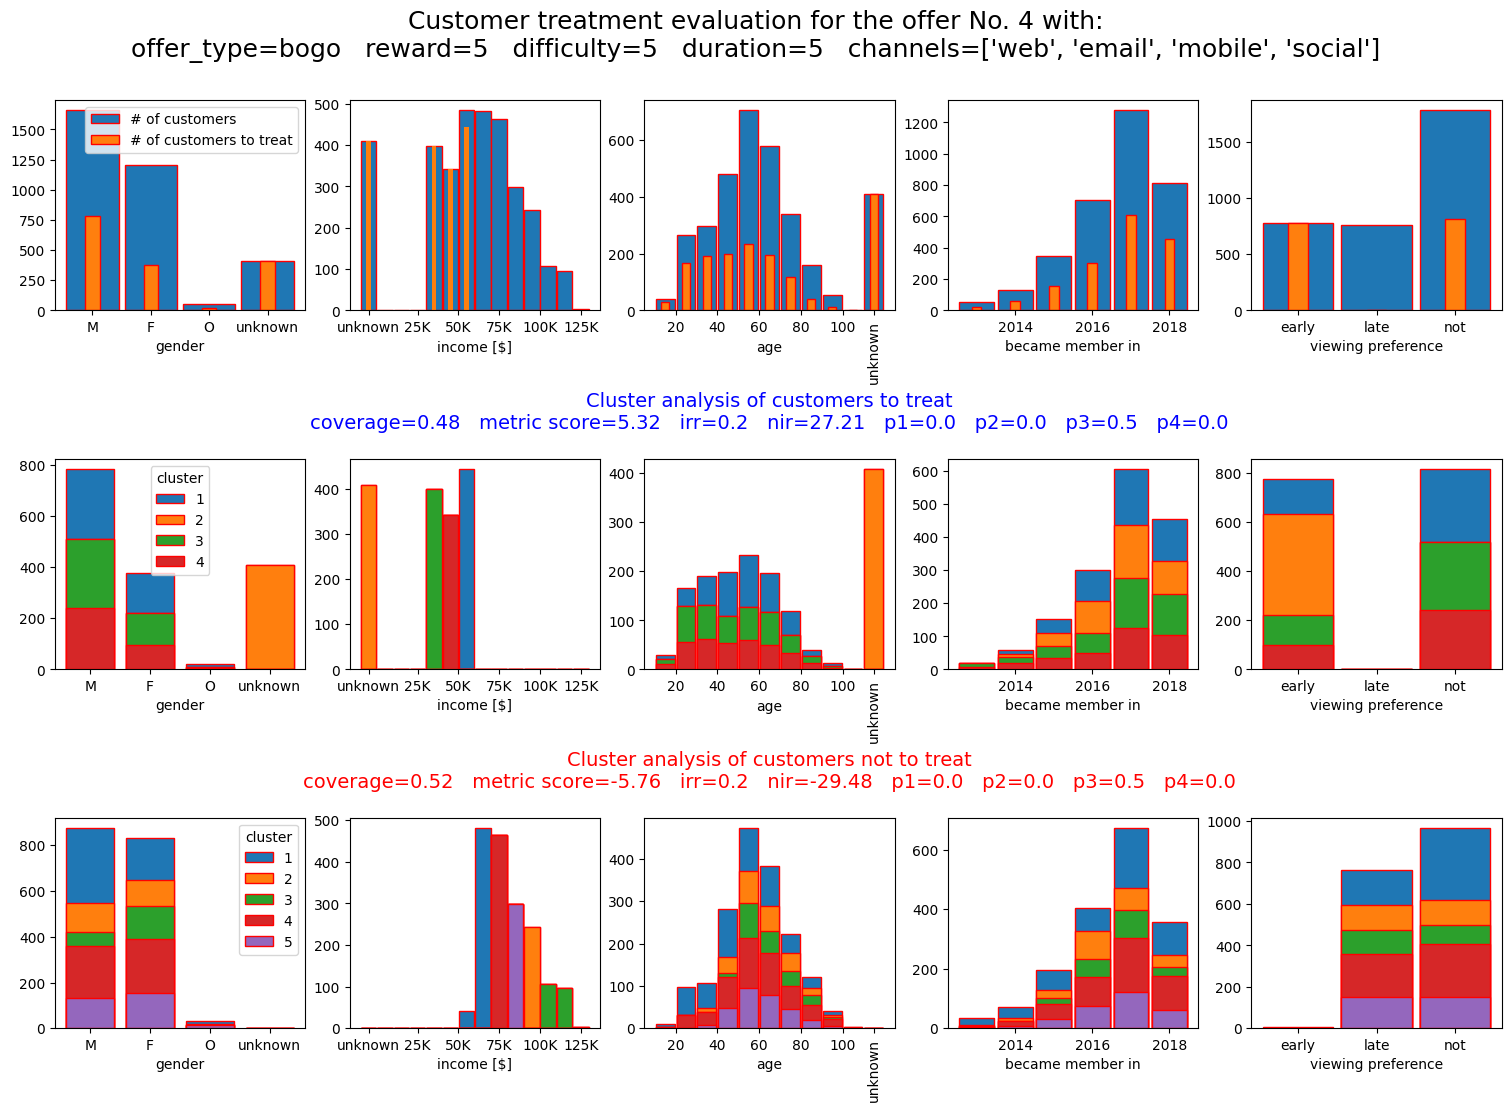
\includegraphics[height=0.5\textheight]{results/results4.png}
\caption{Customers worth targeting with this offer are basically the same as in offer type 2. However, this offer type has a stronger value in the metric score.}
\end{figure}
\subsubsection{Diagrams for discount offers}

\begin{figure}[H]
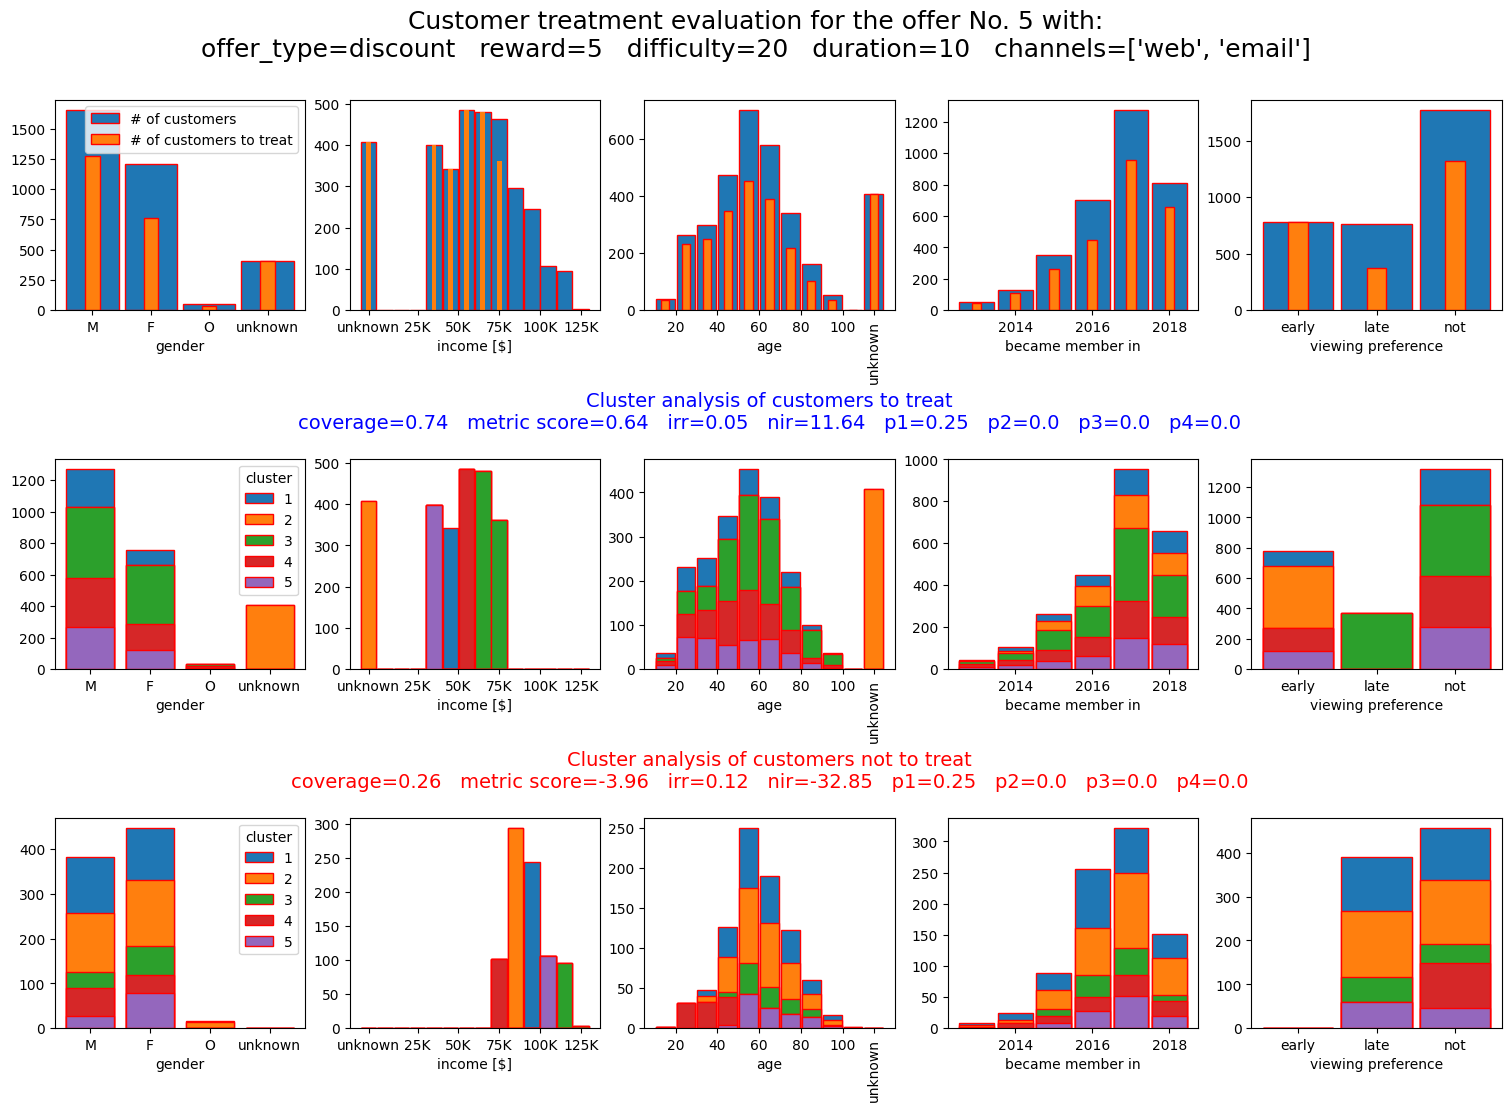
\includegraphics[height=0.5\textheight]{results/results5.png}
\caption{Customers with  incomes up to \$80,000 are worth targeting with this offer. Those who do not provide demographic information should be included as well.}
\end{figure}
\begin{figure}[H]
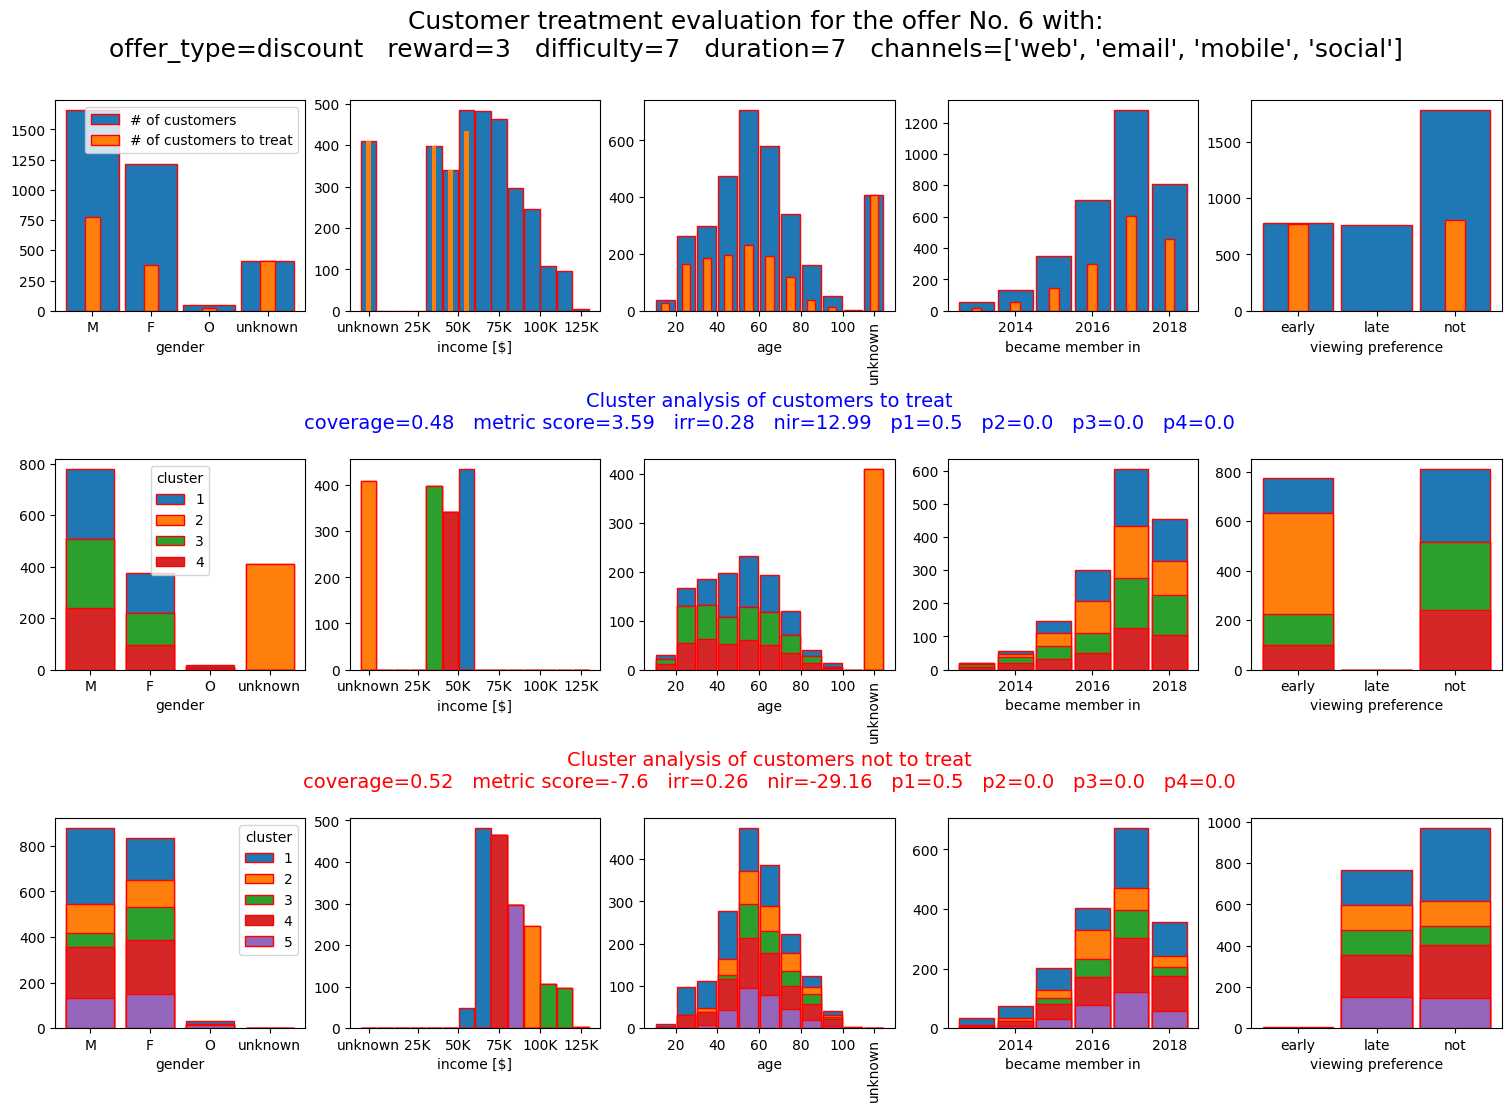
\includegraphics[height=0.5\textheight]{results/results6.png}
\caption{Customers worth targeting with this offer are basically the same as in offer type 2 or 4.}
\end{figure}
\begin{figure}[H]
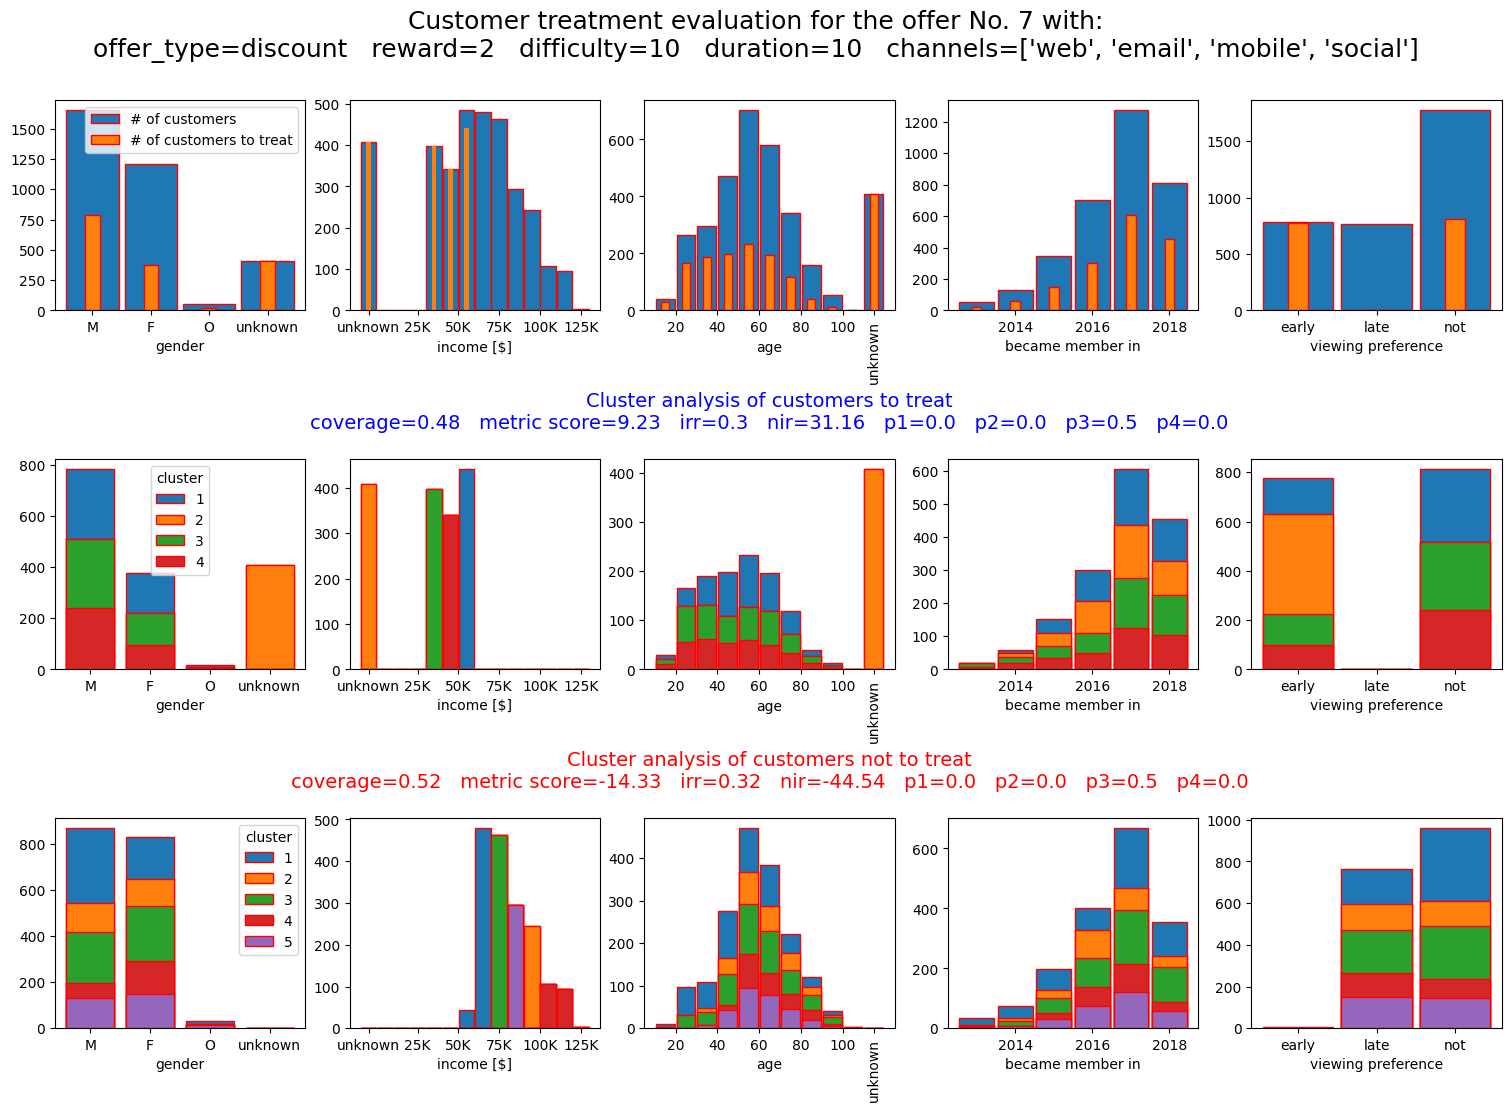
\includegraphics[height=0.5\textheight]{results/results7.png}
\caption{Customers worth targeting with this offer are basically the same as in offer type 2,4 or 6. However, this offer type has a stronger value in the metric score.}
\end{figure}
\begin{figure}[H]
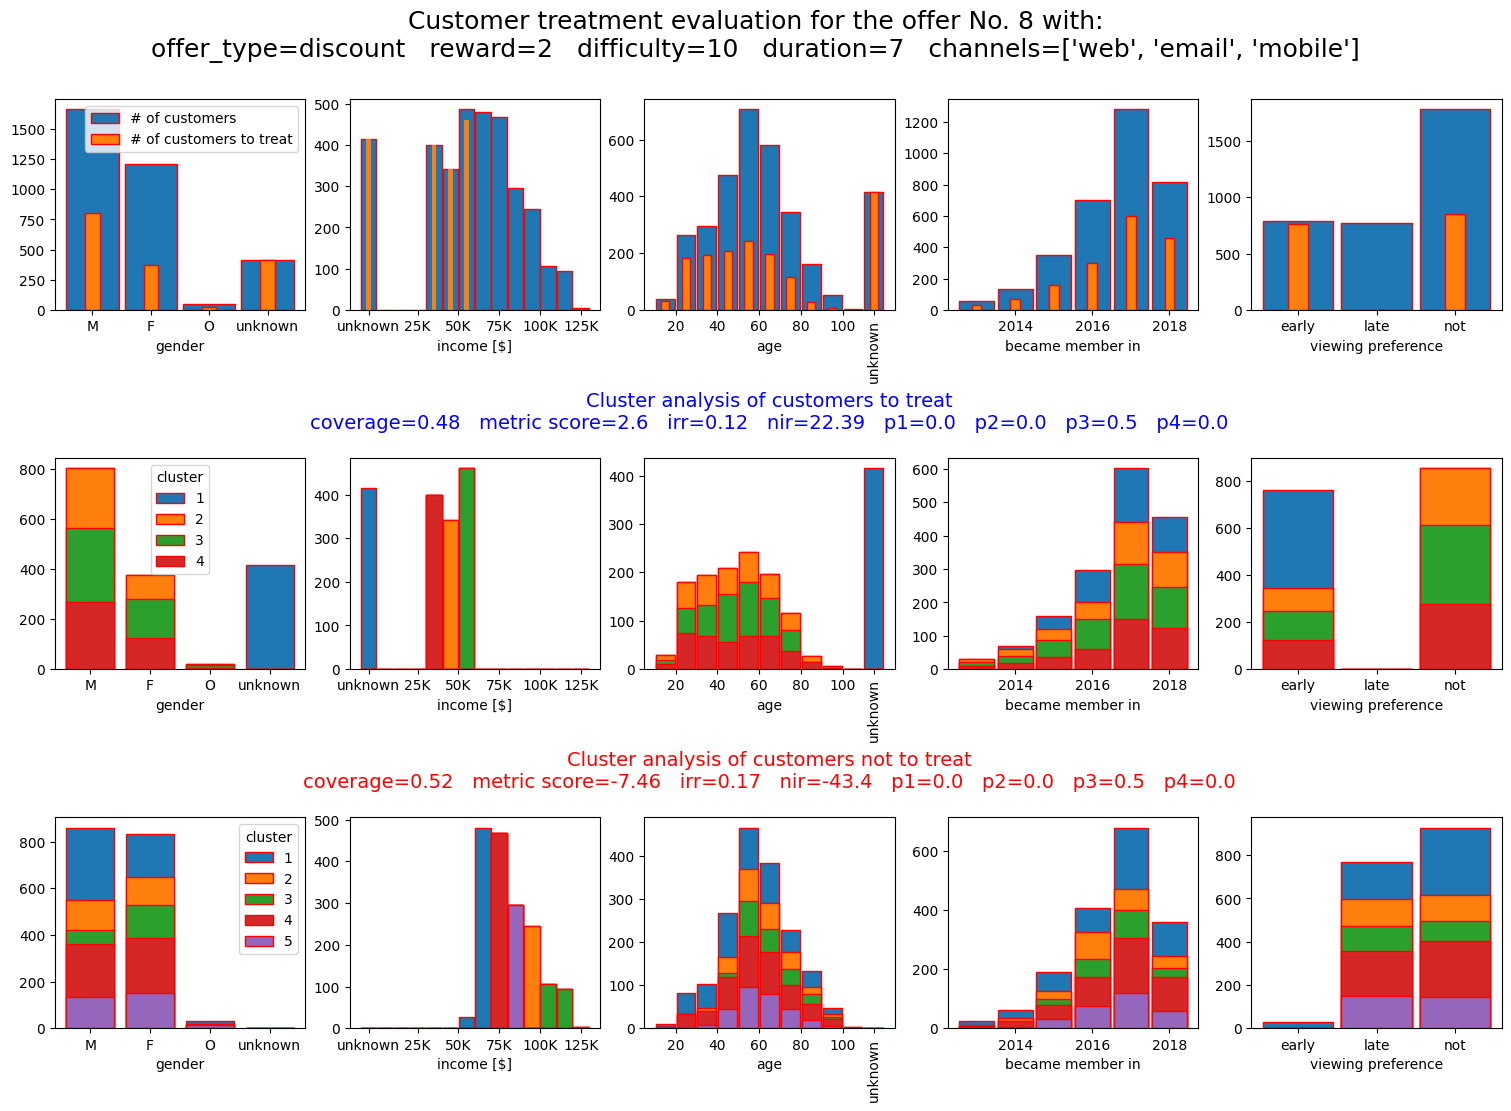
\includegraphics[height=0.5\textheight]{results/results8.png}
\caption{Customers worth targeting with this offer are basically the same as in offer type 2,4, 6 or 7.}
\end{figure}
\subsubsection{Diagrams for informational offers}
\begin{figure}[H]
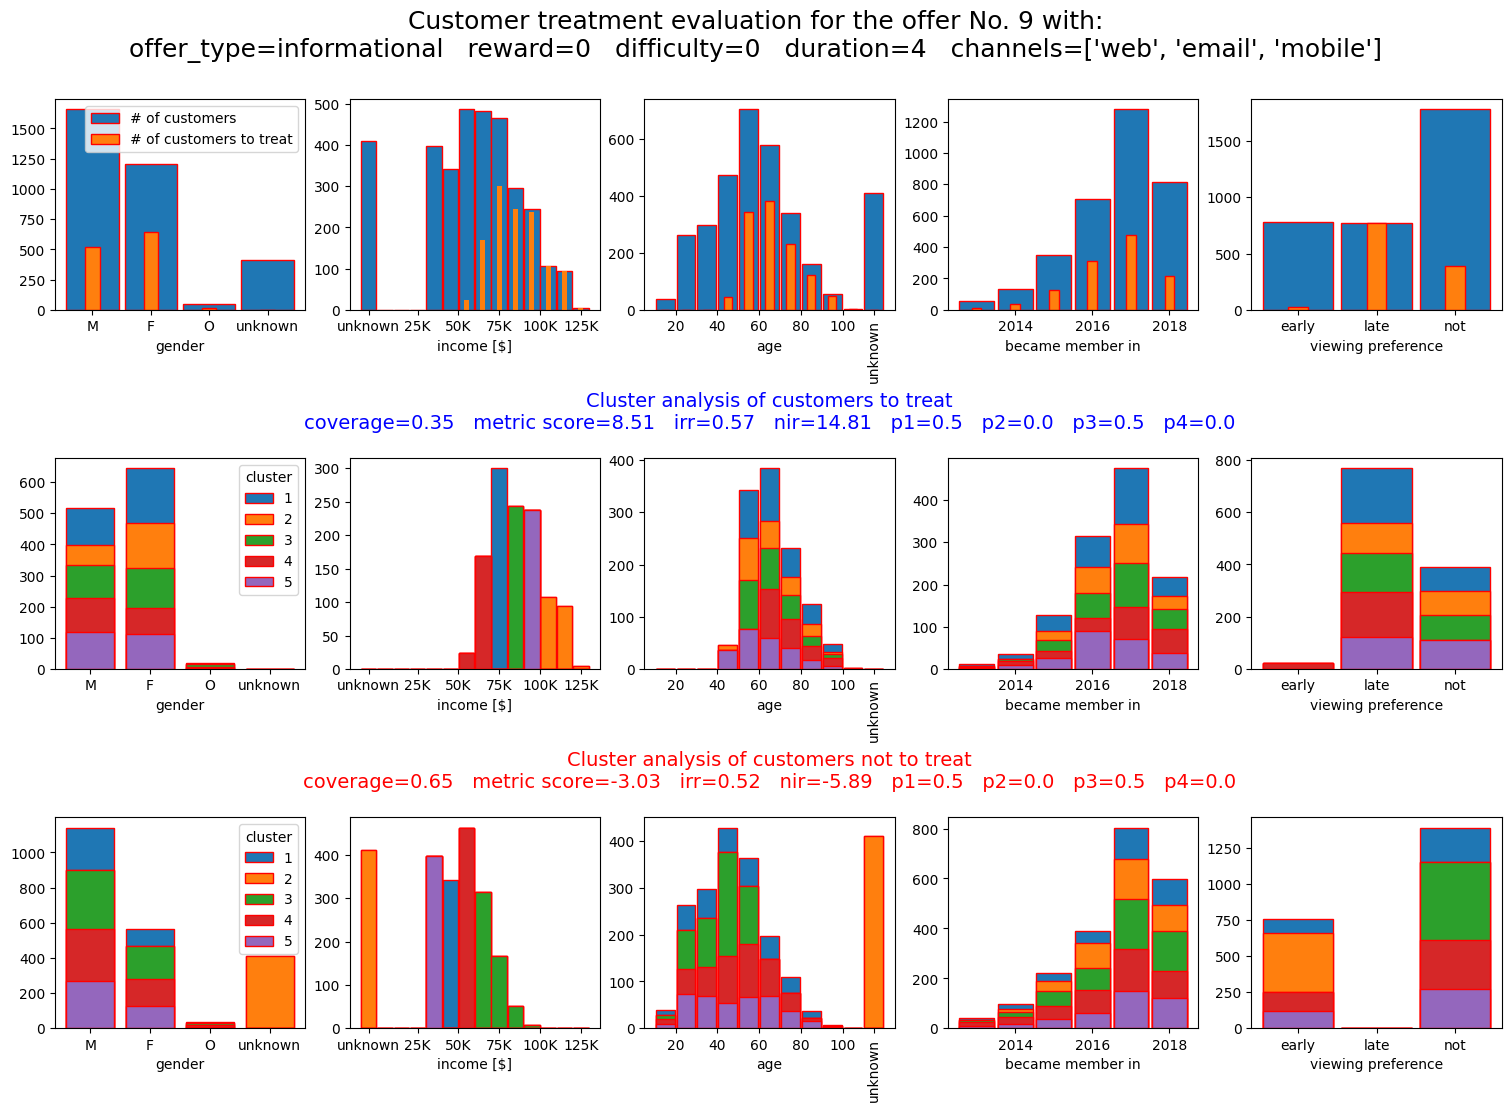
\includegraphics[height=0.5\textheight]{results/results9.png}
\caption{A majority of customers earning at least \$70,000 should be targeted by this offer. These customers are more likely female and tend to view lately or rather not. Customers not providing demographic information should be excluded.}
\end{figure}
\begin{figure}[H]
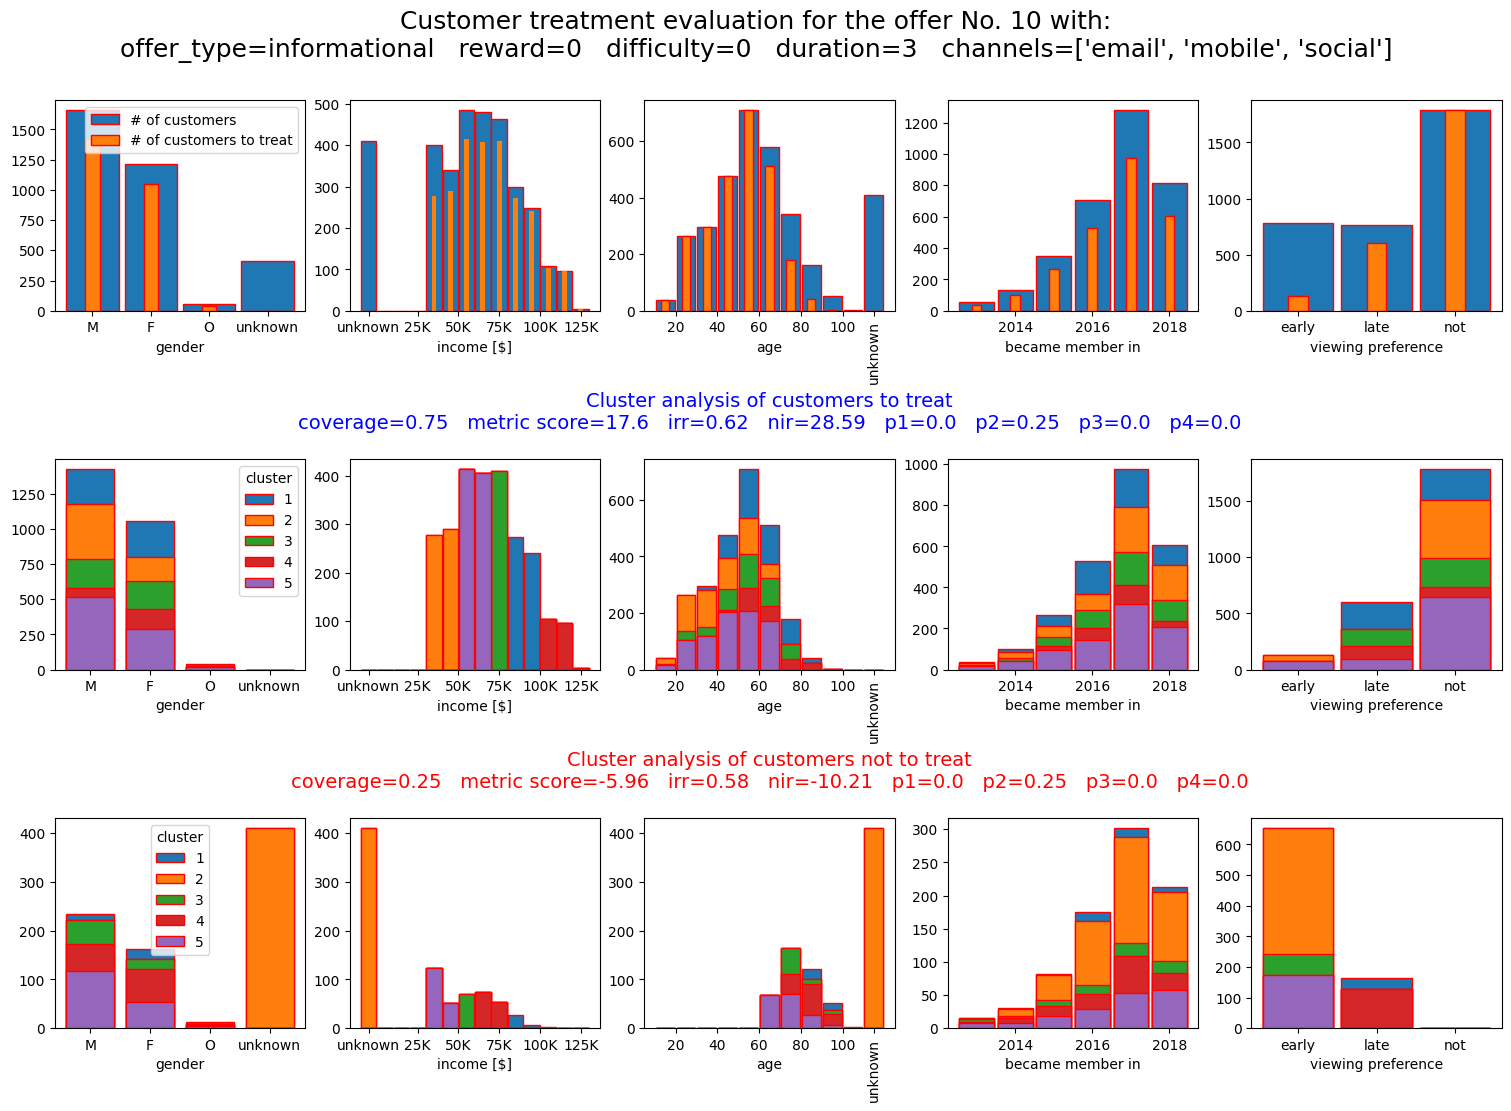
\includegraphics[height=0.5\textheight]{results/results10.png}
\caption{A staggering $75\%$ of customers are worth targeting with this offer, with the highest metric score found. Young and middle-aged customers are particularly worth targets. These customers are more likely to view lately or rather not. Customers who do not provide demographic information should be excluded. Of those with an income of \$60,000 or less, only those who tend to view lately are in the target group.}
\end{figure}


\section{Conclusion}
In this study, we can conclude that BOGO and discount offers are primarily targeted at low- and middle-income customers. The best BOGO offer is offer type No. 4 and is designed for customers earning up to \$60,000.
It has a 5-day validity period and a \$5 threshold. 
The best discount offer is offer type No.~7, which has a 7-day validity period, a \$10 difficulty level and a \$2 reward.
Offer type No.~4 is also designed for customers earning up to \$60,000, but has a metric score that is twice as high as the best BOGO offer.
Nonetheless, both the BOGO and discount offers do not target higher income customers.
On the other hand, we can see that the information offers are intended for high income customers who do not tend to look at offers immediately.
In contrast to the other types of offers, customers who do not provide demographic information are not included in the target group.
It may be that people who do not provide any information about themselves do not want to be informed by the app without any direct benefit.
In fact, the second information offer (offer type No.~10) with the 3 day duration has even the highest metric score of all offers and a coverage of $75\%$.
This seems to be the best choice of offer to send for most customers who provide demographic information.
The remaining customers should receive offer No.~5 or 7 depending on their demographics.
However, it is difficult to make an exact decision within the scope of this research, as a finer screening of the parameters and more data would probably provide more clarity.
With regard to the choice of demographic attributes for a possible promotion decision, we can say that the starting date of membership does not seem to be very characteristic, at least when looking at the year.
However, the impact of the "income" attribute, as well as the decision to provide demographic data at all, seems to be very profound in this context.
There may also be a tendency for targeting via social networks to increase the metric score.




\end{document}
